\subsection{Recapitulació de les tecnologies pel desenvolupament web}

    \paragraph{}
    Els apartats anteriors d'aquest apartat de la memòria s'han utilitzat per explicar i justificar les diferents tecnologies que formen part de la nostra aplicació web.

    En total, es tracta de nou tecnologies que han hagut de ser estudiades per separat i aprés a utilitzar de forma conjunta. L'única tecnologia sobre la qual es disposava en certa forma, d'un petit coneixement previ, era la tecnologia Javascript.

    Es va dedicar una part important del temps destinat al projecte a aprendre a utilitzar tot aquest conjunt de tecnologies, però creiem que el resultat ha estat bastant satisfactori.

    El mapa de tecnologies i el paper que juga cada una d'aquestes en l'arquitectura de capes proposada, es pot veure representada a la figura~\ref{fig:finalTech}.

    \begin{figure}[h]
        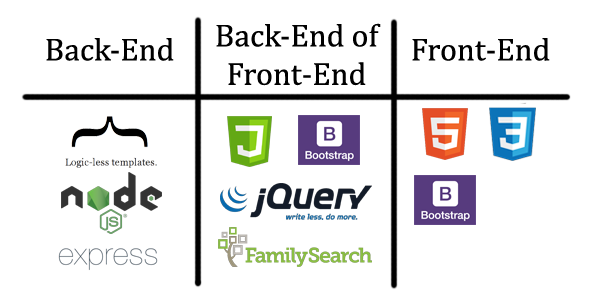
\includegraphics[scale=0.6]{08/05_techFinal}
        \centering
        \caption{Mapa final de tecnologies en cada capa de l'aplicació}\label{fig:finalTech}
    \end{figure}
